\section{Decoding Failure Rate of QC-MDPC Codes}

\subsection{Motivation}

\begin{frame}{BIKE}

BIKE (\textbf{B}it-\textbf{F}lipping \textbf{K}ey \textbf{E}ncapsulation) is based on QC-MDPC (\textbf{Q}uasi-\textbf{C}yclic \textbf{M}oderate \textbf{D}ensity \textbf{P}arity \textbf{C}heck) binary linear codes.

\begin{itemize}
    \item Round 4 candidate in NIST's PQC Standardisation process.
    \item Among the selected algorithms after round 3, 3 are lattice-based, 1 hash-based.
    \item Three algorithms remain for consideration: BIKE, Classic McEliece, HQC, \sout{SIKE}\footnote{SIKE (or SIDH) has been broken in last summer, by Castryk-Decru, Maino-Martindale, Robert, etc.}.
\end{itemize}
    
\end{frame}

\begin{frame}{Motivation}
\begin{itemize}
\item BIKE uses an iterative bit flipping decoder which is not characterized by bounded decoding radius $\implies$ we expect nonzero DFR (\textbf{D}ecoding \textbf{F}ailure \textbf{R}ate).
    \item The security proof of BIKE in the IND-CCA2 setting assumes a low DFR. Currently, DFR has been estimated through simulation and extrapolation.
\end{itemize}
\end{frame}

\begin{frame}{Motivation (cont.)}
\begin{columns}
\column{0.4 \textwidth}
\begin{itemize}
    \item May underestimate DFR due to error floor phenomenon.
    \item Sufficiently high DFR is vulnerable to GJS \footnote{Q. Guo, T. Johansson, and P. Stankovski. A Key Recovery Attack on MDPC with CCA
Security Using Decoding Errors.} attack for ephemeral keys.
\end{itemize}

\column{0.5 \textwidth}
    \begin{figure}
    \centering
    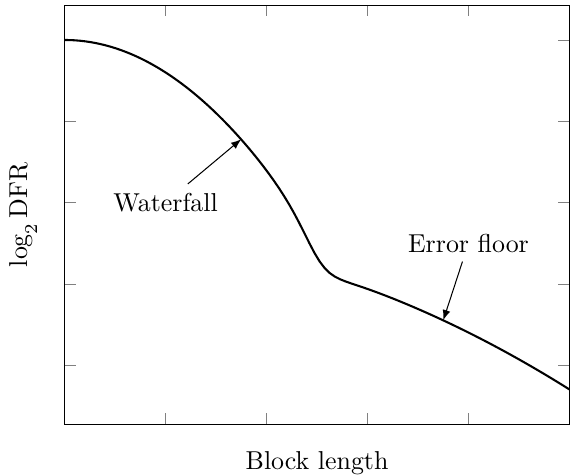
\includegraphics[scale=.2]{Images/errorfloor.png}
    \caption{DFR curve and error floor. Image credit: Valentin Vasseur}
    \label{fig:errorfloor}
\end{figure}

\end{columns}    
\end{frame}